\chapter{Indledning}
Gennem Danmarks fjerde største by Aalborg, løber Limfjorden. Her er Jernbanebroen én af tre overgange, som blev opført i år 1879. Beliggenheden af denne illustreres på Figur 1.1 \citep{redaktionen}. Dengang var det meningen, at der skulle anlægges en vej for både kørende og gående oven på Jernbanebroen \citep{Johannesen}. Vejen over broen blev dog aldrig til noget. Limfjordsbroen blev opført i år 1933, efter et ønske om en forbindelse mellem Aalborg og Nørresundby, der var tilgængelig hele tiden. 
\begin{figure}[htbp]
	\centering
	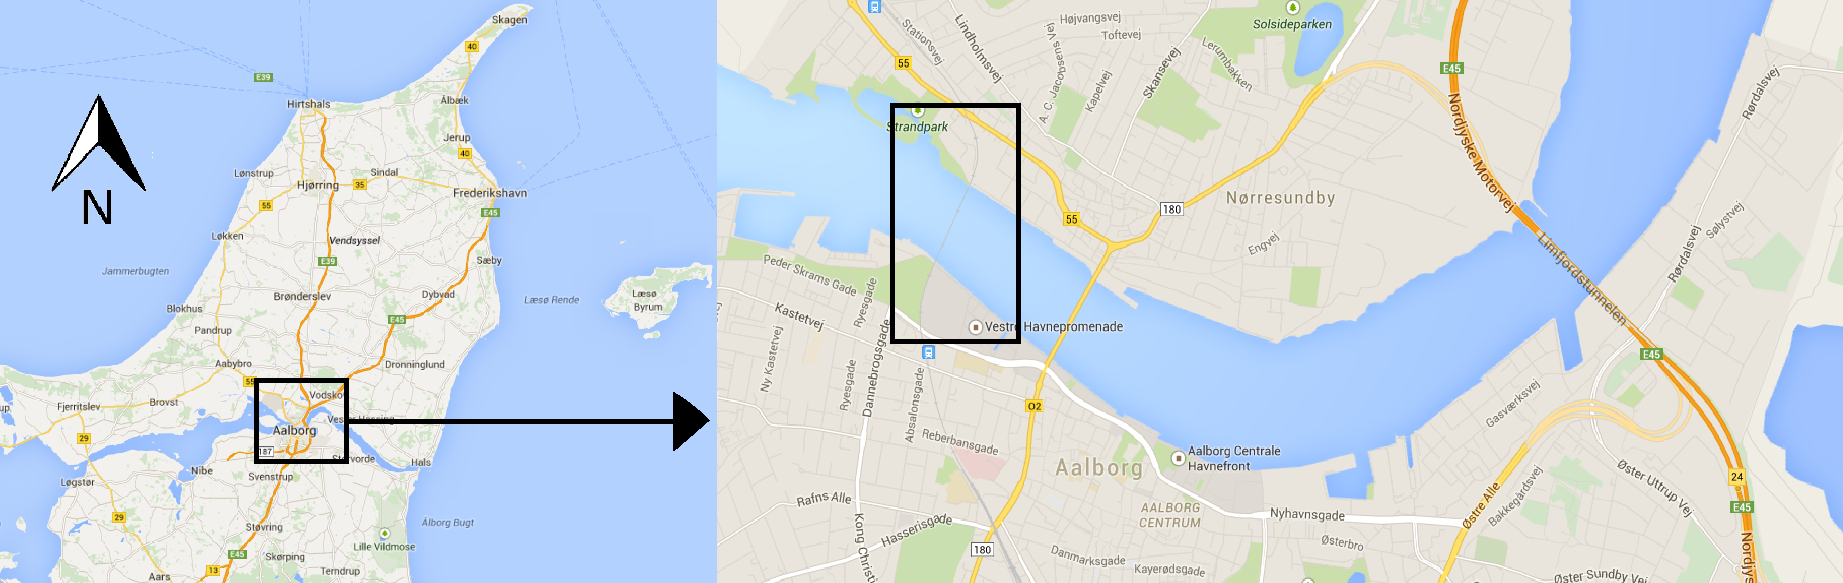
\includegraphics[width=1.0\textwidth]{billeder/indledning1.png}
	\caption{Jernbanebroen over Limfjorden ved Aalborg}
	\label{fig:billede1}
\end{figure}
\newline
De to broer har stået for massevis af menneskers transport over Limfjorden. I 1969 blev der konstrueret en sekssporet tunnel i forbindelse med E45-motorvejen under Limfjorden, som gav bedre mulighed for at køre i bil mellem Aalborg og Nørresundby \citep{DenStoreDanske4} \citep{Vejdirektoratet}.
\newline \indent{     }  Siden Limfjordens tre forbindelsers udarbejdelse har både Aalborg og Nørresundby vokset sig større. Aalborg voksede som by op igennem 1900-tallet, som følge af industrialiseringen, både i størrelse og på indbyggertallet. I 1970 var indbyggertallet i Aalborg cirka 97.000 indbyggere, og i 2014 er dette tal steget til 109.000 indbyggere. I hele Aalborg Kommune er indbyggertallet 205.809 indbyggere og stadig i stor vækst \citep{DenStoreDanske2} \citep{statistik}.
\newline \indent{     }  I takt med at byerne er vokset, er afstanden mellem de yderliggende dele af Aalborg og Nørresundby og ind til Limfjordsbroen blevet større. Gående og cyklister har kun mulighed for at krydse Limfjorden over Limfjordsbroen. Derimod har bilister både mulighed for at krydse ved Limfjordsbroen og gennem Limfjordstunnelen, og ligeledes er det muligt at krydse Limfjorden med offentlig transport; enten med bus over Limfjordsbroen eller med tog over Jernbanebroen.
\newline \indent{     }  Sammen med resten af Nordjylland vokser Aalborg også i dag, hvilket gør betydningen af både Limfjordsbroen, Jernbanebroen og tunnelen vigtige. Særligt Limfjordsbroen er af høj betydning for cyklister og fodgængere, og en eventuel lukning af broen, på grund af reparation eller uforudsete ulykker, ville betyde, at gående og cyklister ikke ville have mulighed for at krydse Limfjorden.
\newline \indent{     }  Det har i flere år været på tale, at bygge en cykel/gangbro på siden af Jernbanebroen. Siden projektets start er der præsenteret tre løsningsforslag. Det første løsningsforslag blev fremlagt i år 2009 af Kærsgaard \& Andersen, der lød på en cykel/gangbro af materialet stål. Tegninger, tekniske mål og udregninger af konstruktionen var lavet, og ligeledes var de første skridt i byggeriet taget, i form af forskellige dele til broen. Grundet en række politiske årsager blev byggeriet sat på standby i 2009, men projektet har fortsat været undervejs. I 2011 præsenterede COWI et nyt løsningsforslag, der lød på en cykel/gangbro af et kompositmateriale af plast og fiber. I år 2013 lød forslaget på et kombiprojekt, der skulle kombinere det oprindelige stålprojekt og det nye glasfiberprojekt \citep{KulturbroAalborg}. 